\documentclass{article}
\usepackage{geometry}
\geometry{
  a4paper,
  left=30mm,
  right=30mm,
  top=20mm
}
\setlength{\parindent}{0pt}
\usepackage{hyperref}
\usepackage{booktabs}
\usepackage{float}
\hypersetup{
    colorlinks=true,
    linkcolor=blue,
    filecolor=magenta,
    urlcolor=blue,
    citecolor=blue,
}
\usepackage{cleveref}
\usepackage{longtable}
\usepackage{graphicx}

\title{Dialogue Practical: Report Phase 3}
\author{Frederik Schittny, Thomas Marwitz}
\date{14 July 2025}

\begin{document}

\maketitle

\section{Implementation Progress}
In the third phase of the project, we strictly followed the improvements identified as most promising in the last phase. A description of the implementation details for each of the improvements is given in the following subsections. The measured system performance and an analysis of the improvements' impacts are given in~\cref{sec:eval}.\\

\begin{figure}[htb]
    \centering
    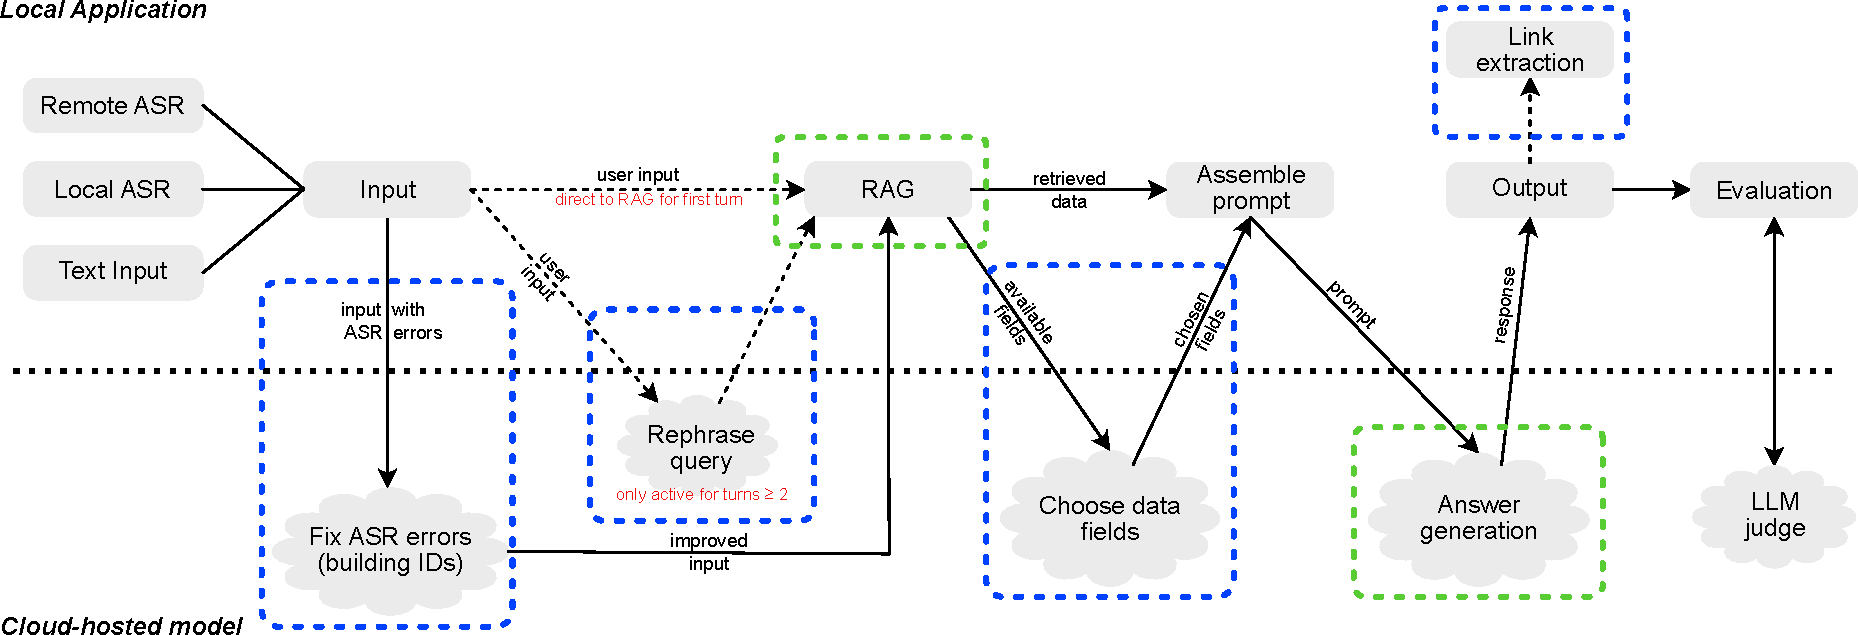
\includegraphics[width=1\linewidth]{data_flow_phase_3.pdf}
    \caption{Data flow chart of the updated system. Components that were added in this phase are highlighted in blue. Existing components that were updated are highlighted in green. Dashed arrows indicate data flow alternatives.}
    \label{fig:data_flow}
\end{figure}

\Cref{fig:data_flow} shows an overview of the implemented system updates. Since we closely followed the plan developed in phase 2, the implemented system closely resembles the planned system from that phase. New components are the ASR fixing (see~\cref{sec:asr_fix}), the data field selection (see~\cref{sec:chosen_fields}), and the query rephrasing (see~\cref{sec:query_rephr}). And the existing RAG component was switched to LlamaIndex (see~\cref{sec:rag_impr}).\\

Before beginning the work on the system improvements, the project was restructured to improve clarity and make the project more comprehensible. Besides relocating files for source code, documentation, and evaluation, the componentization of the system code was improved. Overall, the structure of loosely coupled components that are interfacing via Python protocols made it very easy to implement updates to different system components.

\subsection{ASR Input Fixing} \label{sec:asr_fix}
The fixing of ASR errors is focused on identifying and restructuring numerical building identifiers. While the ASR sometimes correctly transcribes numerical identifiers like "50.34", it often transcribes them in textual form like "fünfzig Punkt vierunddreißig". Depending on the user's pronunciation, different versions of incorrect transcriptions exist for the numerical building IDs. To fix these errors, the ASR-transcribed user input is given to the institute model, which is tasked to identify and correct the errors introduced by ASR.\\

While the overall implementation of an additional model usage in the data flow was easy, designing a suitable prompt for the task proved to be more difficult than expected. Similar to the use case of selecting suitable data fields (cf.~\cref{sec:chosen_fields}), the model was observed to struggle when the language of the data input and the system prompt were not the same. Therefore, the system prompt is written in German, even though the model has probably received more in-depth training for English inputs. The prompt was built around the main idea to provide examples of typical ASR errors for numerical building IDs for in-context learning. However, the model was found to often misinterpret the instructions and try to answer the provided user question, even when specifically told not to do so. Additionally, the model often only returned the fixed segments of the original inputs, instead of the original input with the corrections applied. An attempt at fixing this behavior by reverse prompting based on the few-shot examples with a more powerful Llama 70B model was unsuccessful.\\

Ultimately, the most successful approach proved to be a more structured task for the model to follow. The few-shot examples are given in JSON syntax. The model's task is not to directly replace the ASR errors in the provided input, but to return a JSON dictionary with the identified errors and their corrections. The replacement of the incorrectly transcribed words is then performed via string replacement on the client side. To give the system prompt even more structure, it is provided to the model in markdown syntax. \\

However, we initially underestimated the time cost of generating longer JSON outputs. As the length of the correction list grew, so did the latency significantly. To address this, the output format was changed from full JSON to a more concise, semi-structured list format. This format retains clarity while improving generation speed.\\

In case the model returns an unexpected answer (like incorrect JSON syntax), the system performs a failover to the next processing step. All corrections that were able to be applied up to that point are used by the following system components.

\subsection{RAG Improvements} \label{sec:rag_impr}

\subsubsection*{Evaluating RAG performance gains}\label{subsec:rag-dataset}

The first step in improving the RAG was to construct a simple test set from our initial, comprehensive test set. For each query, we already stored the entity this question relates to. This could be used to generate a RAG test set.

\begin{table}[H]
\centering
\begin{tabular}{|p{10cm}|c|}
\hline
\textbf{User Prompt} & \textbf{Expected ID} \\
\hline
Wo ist Gebäude 30.29? (Where is building 30.29?) & 30.29 \\
Wie komme ich dahin? (How do I get there?) & 30.29 \\
Ist das auch rollstuhlgerecht? (Is it wheelchair accessible?) & 30.29 \\
Wie lange ist das noch offen? (How long is it open?) & 30.29 \\
\hline
\end{tabular}
\caption{Multi-turn conversation test case with expected entity ID. From this, we could generate a simple RAG test set by looking at the first question only.}
\end{table}

To test the RAG component (without the query rephrasing), we simply looked at the first question only, which still constituted 200 cases. Each change could then be tested by retrieving 5 rows (identified by their building ID) and counting how many times the expected ID was among them.

\subsubsection*{Improvements made}

First, we added the `name' column to enrich the data for RAG, allowing the system to find, e.g. the Cafeteria that has a building ID of 01.12. So asking for the cafeteria and only querying the initial ID column would fail to retrieve the correct object. Second, we implemented Reranking with a Cross-encoder model. Third, we choose a `better', more recent model for the intial retrieval, allowing us to improve the retrieval even a bit more. Starting from 170 (of 200) successful retrievals for the baseline RAG, we improved that to 175, 184, and 187, respectively.

\begin{table}[H]
\centering
\begin{tabular}{|l|c|c|}
\hline
\textbf{Enhancement Step} & \textbf{Turn 1 Success (out of 200)} & \textbf{Success Rate (\%)} \\
\hline
Baseline RAG & 170 & 85.0 \\
+ `name' Column for Enrichment & 175 & 87.5 \\
+ Cross-Encoder Reranker & 184 & 92.0\\
+ Improved Initial Retriever Model & 187 & 93.5 \\
\hline
\end{tabular}
\caption{Incremental improvements in Turn 1 retrieval success.}
\end{table}

\subsubsection*{Problems}

Things that didn't work out: Performing RAG over all columns was lowering the signal available to the similarity search. To reap the benefits of the data stored in all columns, a more sophisticated approach like a \href{https://docs.llamaindex.ai/en/stable/examples/query_engine/pandas_query_engine/}{Pandas Query Engine} might work.

The initial ASR Input Fixing idea of just appending the fixed input string the initial query proved to lower the signal, therefore worsening the amount of successfully retrieved rows (entities). Because of the RAG-specific test set, we were able to pinpoint and fix this. Our key takeaway here is that end-to-end tests are nice to recognize gains and losses in overall performance but more specific datasets can serve as `unit tests' which allow for more straightforward investigations in cases of failure.

\subsection{Model-Chosen Data} \label{sec:chosen_fields}
Due to the observation that the model often included more information on a building than is necessary to answer the user's question, we decided to restrict the model's access to unnecessary information. To do so, the retrieved information is filtered before being given to the model for answer generation. This is implemented as an additional LLM query.\\

Similar to the development of the ASR input fixing (cf.~\cref{sec:asr_fix}), several different system prompts were investigated. The overall best approach is essentially the same as for the ASR fixing. The model is prompted to return the fields it deems necessary for answering the provided user question as a JSON array. Several few-shot examples for common user questions are provided in the prompt. The returned JSON array is then used on the client side to filter out all retrieved information that is not needed for answering the user's question. Because the model was observed to adhere more strongly to instructions provided at the end of the prompt, the few-shot examples are provided in order of reversed importance. Additionally, a summarized description of the model's task and a reminder to be restrictive with selected information are provided at the end of the prompt.\\

As with the ASR input fixing (cf.~\cref{sec:asr_fix}), the system continues with an unfiltered input if the model returns an unexpected response, which cannot be used to filter the retrieved information.

\subsection{Query Rephrasing} \label{sec:query_rephr}

\subsubsection*{Problem: Chosen-data fields component breaks multi-turn}
While restricting the model's access during question answering to the necessary data fields, it has the side effect of breaking the system's ability to perform well in multi-turn dialogues. Since many higher-turn questions leave building identifiers like numbers and names to the dialogue context, the system, as implemented in phase 2, is unable to retrieve useful documents. Previously, the model was able to answer a question like "Und wann hat das Gebäude geöffnet?" by attending to the information retrieved in the last turn, which is included in the dialogue history. However, with the new information filter described in~\cref{sec:chosen_fields}, the needed information can neither be retrieved nor taken from the dialogue history.

\subsubsection*{Solution: Dedicated Component}

To fix this issue, a prompt rephrasing step was added, which enriches higher-turn user queries with context from the dialogue history. For every follow-up user input, a model call is performed, which queries the model to add the information necessary for a retrieval (e.g. building names or numbers) to the input before the retrieval is performed. This not only re-enables the system to handle multi-turn scenarios. Compared to the previous implementation, where the model had to realize the useful information was provided in the dialogue history instead of in the retrieval of the current turn, this update makes sure that the information most relevant for answering a question is always retrieved in the same turn.

\subsubsection*{Re-using the RAG-specific dataset for direct component evaluation}

Again, we could use our specific dataset from \ref{subsec:rag-dataset} to evaluate the improvement of our component more directly than in an end-to-end test. Only this time, we looked at the follow up turns and their retrieval success.

\begin{table}[H]
\centering
\begin{tabular}{|c|c|c|c|}
\hline
\textbf{Turn} & \textbf{Before Rephraser} & \textbf{After Rephraser} & \textbf{Difference} \\
\hline
Turn 2 & 0.04 (8/200) & 0.91 (182/200) & +0.87 \\
Turn 3 & 0.08 (11/132) & 0.97 (128/132) & +0.89 \\
Turn 4 & 0.09 (6/65) & 0.98 (64/65) & +0.89 \\
\hline
\end{tabular}
\caption{Success ratios before and after Rephraser (Turn 2 and later)}
\end{table}

% Due to ASR-input / RAG clash input fixing, not enough time to adjust the system prompt
% \subsection{Updated System Prompt} \label{sec:system_prompt}
% \textcolor{red}{Add description of changes to the system prompt here. Also describe things that might not have worked but were explored as options.}

% \subsection{Link Extraction} \label{sec_link_extr}
% \textcolor{red}{remove this if no time for implementation (also from the data flow chart)}

\subsection{Intent Classification}
Because the comparatively small Llama model used in the system struggled with long and complex instructions, we developed the idea to break up the system's tasks into distinct intents. Different kinds of questions could be identified by an additional model query and classified as intended, like building location, opening hours, wheelchair accessibility, and general conversation. The experimental implementation for this intent classification also included one intent for restricted questions, for which the system was supposed to refuse an answer politely.\\

While functionally the experimental implementation of intent classification worked well, the overall idea was found to restrict the system too much. The intent classification would allow the formulation of shorter and more precise system prompts for each intent, which would be easier for the model to follow. However, any user question that would not fit well into any of the pre-defined intents would highly impact the system's performance. A simple example for this is a question that asks for both the location and opening hours of a building. Since the system would only classify the intent as either building location or opening hours, the system would likely only partially answer the user's question. Due to this limitation, the intent classification was scraped after the experimental implementation.

\section{Evaluation} \label{sec:eval}
% \textcolor{red}{Als Hauptabbildung ein Barchart wie wir es schon bislang verwendet haben. WICHTIG: explizit anmerken, dass wir immer nur die Performance des gesamten Systems iterativ evaluieren, also mit jedem neuen Balken eine Verbesserung dazukommt (damit man nicht denkt, die Evaluation wäre immer gegen die Baseline aus Phase 2)}\\

% \textcolor{red}{Außerdem einmal LLM as a judge und die dabei erstellten Messgrößen nochmal etwas detaillierter beschreiben, um auf die Anmerkunngen aus dem letzten Bericht einzugehen. (system prompt für LLM judge ggf. in den Appendix)}

Individual test cases developed for specific components were already discussed to highlight potential problems or improvements found during development. Furthermore, they underscore why certain design decision were made.\\

Apart from individual, ad-hoc developed evals, we evaluate our system again in a systematic manner. We discard the BERTScore metrics that were gathered in the previous report as we found little correlation with overall system performance. Instead, we only use an LLM Judge equipped with the powerful `Qwen3-32B' under-the-hood. Each answer of our system is compared against an expected output and is assigned a score between 0 and 1, in addition to a pass or fail decision. In \ref{fig:overall_perf}, the metrics represent an average of the score across all single / multi / ASR interactions and in \ref{fig:single_turn_perf} an average across the individual categories.


\subsection{Evaluation Strategy: Cumulative Component Integration}

To evaluate system performance, we adopted a cumulative strategy where each new component builds upon the previous ones, resulting in progressive configurations:
\begin{itemize}
    \item Baseline means system at the end of phase 2
    \item \#1 means Chosen Fields
    \item \#2 means \#1 + Better RAG Model
    \item \#3 means  \#1 + \#2 + ASR Fixing
\end{itemize}

This incremental layering approach offers two key benefits. First,
\textbf{Entanglement Awareness}: Since components are interdependent (e.g., ASR fixing might hurt RAG), isolating them can be misleading. Evaluating them in context ensures practical relevance. And second, \textbf{Clarity in Overall Gains}: Rather than disentangling marginal contributions, this strategy provides a clear picture of end-to-end system improvements at each step. Furthermore, it is only logical to compare these components against the baseline by building up on the baseline. Our cumulative testing aligns well with this paradigm.


\subsection{Results}

Our goal in this phase was to integrate the three outlined components as we reasoned they can improve the system performance measureably. The bar to clear was therefore an overall system performance gain with each component integrated. While we used local ASR to pre-transcribe audio in the second phase, this time, the evaluation was carried out against the institute's ASR. The results are satisfying as they confirm our goal to continously improve the system. Still, there is some room left to improve.

\begin{figure}[H]
    \centering
    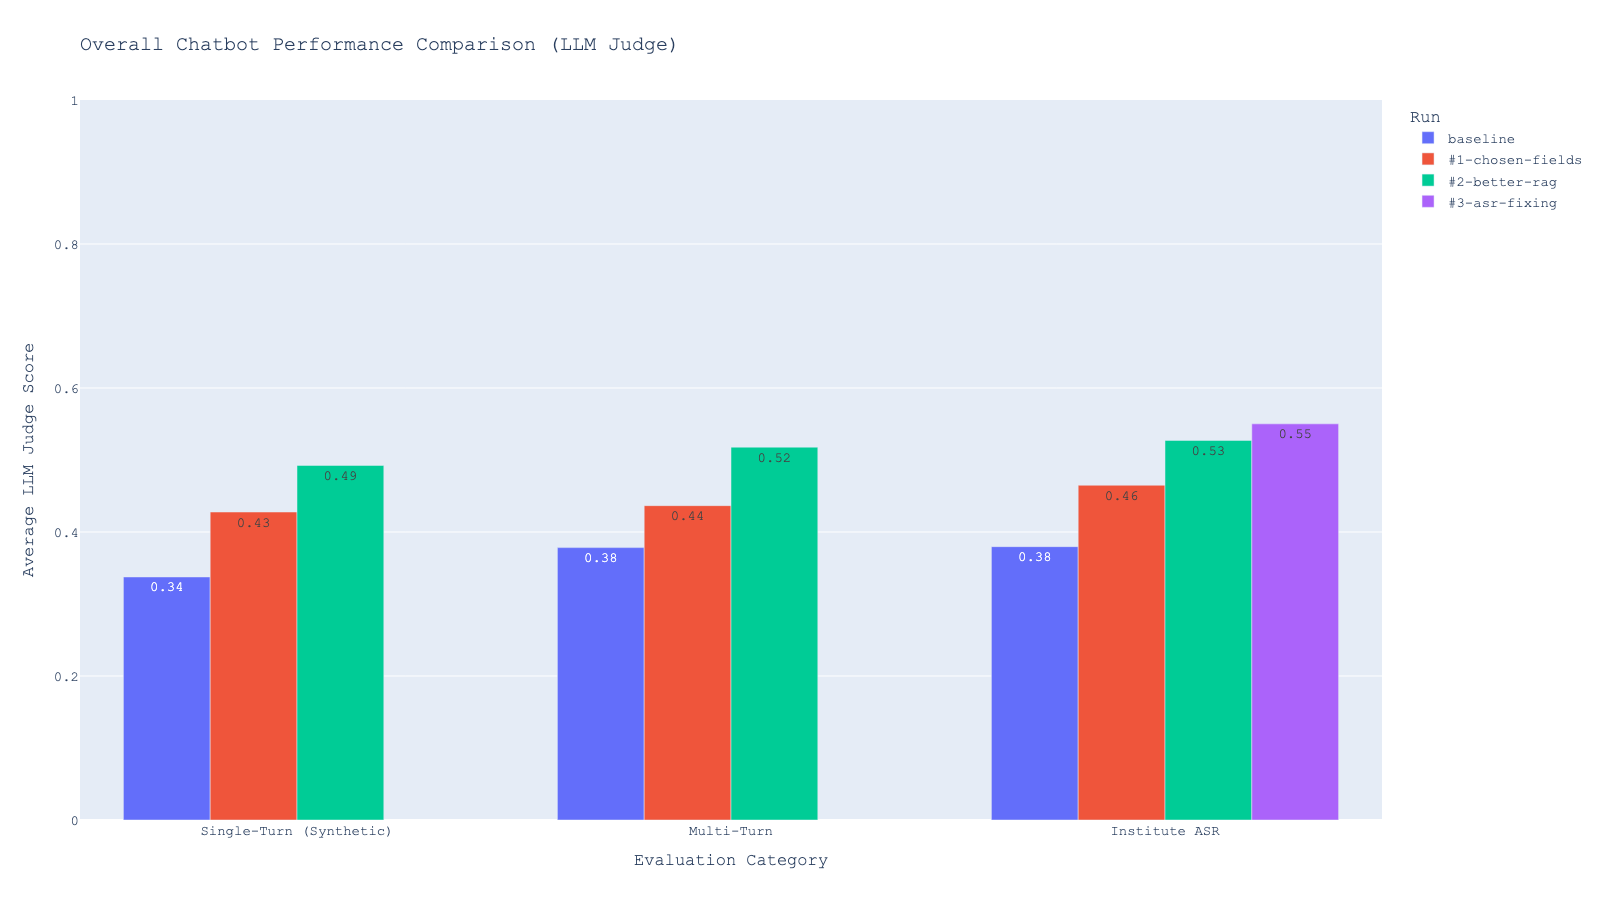
\includegraphics[width=1\linewidth]{overall_performance_comparison.png}
    \caption{The overall performance across single-, multi-, and transcribed turns. The score displayed per chart is the average across the LLM Judge's score across the three categories.}
    \label{fig:overall_perf}
\end{figure}

\begin{figure}[H]
    \centering
    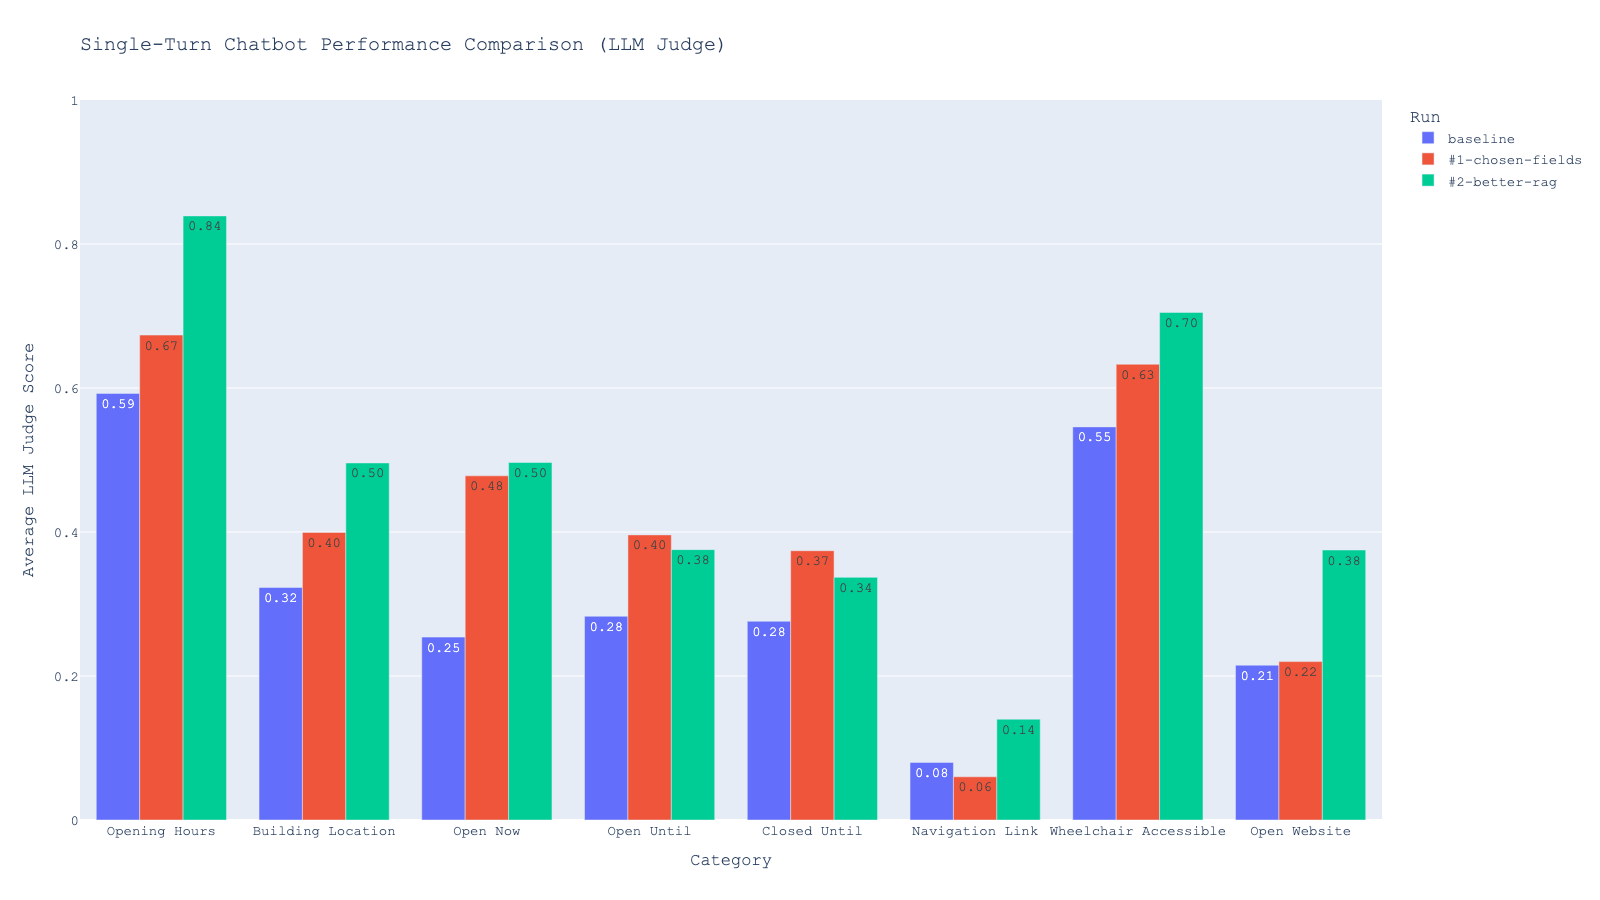
\includegraphics[width=1\linewidth]{single_turn_performance_comparison.png}
    \caption{The overall performance across categories (single-turn). The score displayed per chart is the average across the LLM Judge's score across the individual question categories.}
    \label{fig:single_turn_perf}
\end{figure}

\subsection{Case Study: Evaluating the effect of component \#1 in more details}

What options do we have to evaluate a component other than running our full-fledged end-to-end tests? Of course, we can do "vibe" testing by interacting with our system a dozen times and see how the interaction "feels". However, this is neither feasible nor is it quantifiable. That's where the reason string of the LLM Judge comes into play. For each assigned score, the LLM Judge gives a reason for its rating (see \ref{subsec:llm-judge}. On an individual basis, this might not be so interesting, but the interesting trends are revealed when aggregating across these data points. In \ref{tab:conciseness}, we aggregate over all reason outputs across all evals for the baseline and the data picker component. The results paint a clear picture regarding how the system "feels".

\begin{table}[H]
\centering
\begin{tabular}{lrr}
\hline
\textbf{Keyphrases} & \textbf{baseline} & \textbf{\#1-chosen-fields} \\
\hline
Additional Information & 131 & 60 \\
Unnecessary Detail     & 80  & 40 \\
Unrelated Information  & 30  & 7  \\
Extra Information      & 42  & 10 \\
\hline
\end{tabular}
\caption{Amount of keyphrases across all `reason' outputs of LLM judge. We see a clear improvement regarding conciseness.}
\label{tab:conciseness}
\end{table}

\subsection{Case study: Considering timing trade-offs in component \#3}

When developing an end-to-end system, you have to consider the different dimensions a change will impact your system. Also, you have to consider whether the `improvement' is not breaking any previous available behavior. One dimension we also evaluated here is the average time the additional component ASR fixing costs us, in terms of how fast the user receives an answer.

In this specific case, the way that ASR fixed input was provided (`Initial ASR fixing') to the RAG component made the general RAG worse, while the "relevant" targets (queries with numbers in them) improved. After this trade-off could be resolved (in `Fixed RAG ASR fixing'), analyzing the time spent on fixing ASR errors revealed further optimization potential by reducing the output to a minimum (in `Short output ASR fixing').

\begin{table}[H]
\centering
\begin{tabular}{|l|c|c|c|}
\hline
\textbf{Type} & \textbf{\% Correct (relevant)} & \textbf{\% Correct (Total)} & \textbf{Avg. Time (s)} \\
\hline
Baseline (no ASR fixing) & 0.74 (68/92) & 0.58 (106/182) & 0.00 \\
Initial ASR fixing       & 0.82 (75/92) & 0.51 (93/182)  & 1.71 \\
Fixed RAG ASR fixing     & 0.84 (77/92) & 0.64 (116/182) & 1.71 \\
Short output ASR fixing  & 0.85 (77/92) & 0.64 (116/182) & 0.38 \\
\hline
\end{tabular}
\caption{Retrieval Success for ASR fixed input, all input and time taken to run the ASR fixing. Relevant means that there were building numbers present in the query. This highlights two important lessons learned: a) ensure the component is actually improving the overall performance without breaking anything and b) accuracy or success probability is not the only relevant metric to consider, in an interactive system, response time should be considered as well.}
\end{table}

% \begin{itemize}
%     \item Each system update was evaluated against the current system (with all other updates included)
%     \item Bar to clear for each update was to improve overall system performance
%     \item Pre-transcribed ASR inputs used for intermediate evaluation. Institute ASR used for final (full) system evaluation
%     \item Discussion of the improved performance for each update to the system
%     \item For RAG, there can be an extra discussion for retrieval accuracy (including improvements with rephrasing for multi-turn) $\rightarrow$ add a dedicated chart for that
%     \item Small measurement of latency increase on a few sample prompts
% \end{itemize}

\subsection{Detailed Information: LLM as a Judge}\label{subsec:llm-judge}

\href{https://ai.pydantic.dev/evals/#evaluation-with-llmjudge}{Pydantic AI}'s framework was used to construct the judge. There, a `rubric'is given to the judge s.t. a focus can be set for the evaluation. Apart from that, the LLM is instructed to rate the answer, provide a binary pass rating, and reasoning in form of a string, all packed into a json.

\paragraph{Judge's input}
This is copied from the source code of Pydantic Ai, to help understand how our eval was setup. Given an input (user question), an expected output (from our comprehensive test set), an actual output (llm generated answer), and the rubric (shown below) to set a focus during grading, the judge produced a grading output.
\\
\\
Input:
\begin{verbatim}
    user_prompt = dedent(
        f"""
        <Input>
        {_stringify(inputs)}
        </Input>
        <ExpectedOutput>
        {_stringify(expected_output)}
        </ExpectedOutput>
        <Output>
        {_stringify(output)}
        </Output>
        <Rubric>
        {rubric}
        </Rubric>
        """
    )
\end{verbatim}

Output spefication:
\begin{verbatim}
    You are grading output according to a user-specified
    rubric. If the statement in the rubric is true, then
    the output passes the test. You respond with a JSON object with
    this structure: {reason: string, pass: boolean, score: number}
\end{verbatim}


\paragraph{Judge Prompt for Single-Turn Rating}
\begin{verbatim}
Output should match expected output in meaning, however,
phrasing or wording can differ if the same information is
conveyed. It is mandatory the information is conveyed
instead of listing excuses. The chatbot has access to the
underlying data if the expected output also contains information.
When evaluating addresses, it is okay if the response only
includes the relevant address (street and house number)
as we expect all users to be based in Karlsruhe, Germany.
Reasoning should be concise and to the point. Format your
output as valid JSON object with valid quotation marks. /no_think
\end{verbatim}


\paragraph{Judge Prompt for Multi-turn Rating}
\begin{verbatim}
This is an evaluation of a multi-turn conversation.
The user input is the latest prompt in a conversation.
The full conversation history up to the current turn
is provided as part of the input.
The output is the chatbot's latest response.
The expected output contains the information that
should be conveyed in the response.

Please evaluate if the chatbot's response is coherent
and relevant given the full conversation context.
Focus on the last answer within the total context.
The output should match the expected output in meaning,
however, phrasing or wording can differ if the same
information is conveyed.
It is mandatory that the information is conveyed
instead of listing excuses.
The chatbot has access to the underlying data if the
expected output also contains information. When evaluating
addresses, it is okay if the response only includes the
relevant address (street and house number) as we expect
all users to be based in Karlsruhe, Germany.
Reasoning should be concise and to the point.
Format your output as a JSON object with
valid quotation marks. /no_think
\end{verbatim}

\subsection{A clear look: Binary Pass / Fail Overview}

We evaluated the system for component 1 and 2 on all single turn data and display the amount of passed testcases. This is a sensible way to look at the system to see how many answers were `acceptable'.

\begin{table}[H]
\centering
\begin{tabular}{|l|c|c|c|c|}
\hline
\textbf{Category} & \textbf{Test Cases} & \textbf{Baseline} & \textbf{\#1} & \textbf{\#1 + \#2} \\
\hline
Building Location     & 85  & 19  & 30  & 40 \\
Closed Until          & 100 & 24  & 35  & 31 \\
Navigation Link       & 50  & 0   & 0   & 0  \\
Open Now              & 100 & 20  & 44  & 45 \\
Open Until            & 100 & 21  & 35  & 33 \\
Open Website          & 100 & 17  & 20  & 34 \\
Opening Hours         & 100 & 53  & 62  & 81 \\
Wheelchair Accessible & 100 & 49  & 60  & 68 \\
\hline
\end{tabular}
\caption{Single-turn test results. The LLM Judge assigns a binary attribute `pass' for each test case. We display per category how many of the test cases passed.}
\end{table}

\begin{table}[H]
\centering
\begin{tabular}{|l|c|c|c|c|c|}
\hline
\textbf{Category} & \textbf{Test Cases} & \textbf{Baseline} & \textbf{\#1} & \textbf{\#1 + \#2} & \textbf{\#1 + \#2 + \#3} \\
\hline
ASR Test Set & 248 & 79 & 109 & 114 & 120 \\
\hline
\end{tabular}
\caption{ASR test results including ASR Fixing (\#3). The LLM Judge assigns a binary attribute `pass' for each test case. We display per category how many of the test cases passed.}
\end{table}

\section{Discussion}
As has become evident by the evaluation in~\cref{sec:eval}, the system's performance substantially improved over the baseline performance of the MVP from project phase 2. Therefore, the goal of the third phase, which was to improve the system's performance by implementing the proposed system updates, has been successfully achieved. It is especially noteworthy that each of the originally proposed updates measurably improved the system's performance. While not all updates achieved equal levels of improvement, this positively reflects on the error analysis performed at the end of the second phase.\\

On the other hand, it is important to acknowledge the fact that the current implementation is far from working perfectly. Besides an imperfect implementation, this might also be partly due to the evaluation process. Since limited resources were available for the implementation and evaluation of the system, the test set that was created in the first phase and the adoption of LLM-as-a-judge in the second phase are reasonable and, to a certain degree, suitable measures for evaluating the system. However, neither the evaluation itself nor the test set it is based on were created from actual user data. The system's improved performance on the available test set likely reflects an increased usability for real-world users. This was also anecdotally observed during the implementation of the system improvements. But the exact degree of usability cannot be accurately determined without user feedback from a relevant target group.\\

At this point, the most obvious issues that were identified in the MVP have been addressed. This means that the system is ready to be further evaluated and analyzed based on feedback from a small group of early testers. We will implement a simple graphical user interface in the final phase of the project. While this will help improve the system's ease of use for a potential user evaluation, we will be unable to perform such a beta test due to time constraints.

\section{Future Developments}
As mentioned before, we will be unable to implement further substantial improvements to the system's performance due to time constraints. In the following, we describe several next development steps that we deem to be useful but will be unable to implement.\\

The recent system improvements include fixing errors in numerical building identifiers introduced by the ASR. This measure has improved retrieval of relevant building information. The ASR has also been observed to incorrectly transcribe many of the German proper names of buildings (e.g. Engler-Bunte-Hörsaal). Being able to correct transcription errors in proper names would further increase RAG performance. However, the fixing of proper names is more complex, since the errors can not be described by a set of common mistakes. The currently best idea is to provide the model with a list of available proper names to identify potential mistranscriptions based on similarity to names from the list. The downside of this approach is that it cannot adapt to new proper names without also expanding the reference list. This would make the approach less flexible than the correction of numerical building IDs, which is based entirely on a low number of few-shot examples.\\

The query rephrasing component was not planned as part of the system improvements after the end of the second phase. It was only added in the first phase, after it became apparent that filtering the retrieved data to only include necessary data was breaking the system's multi-turn abilities. This leads to the ASR fixing and the query rephrasing to be to separate steps implemented as two separate queries to the model. Integrating these two distinct processing steps into one could have several advantages. Even though system latency is not a big issue overall, one less interaction between the client side and the cloud-hosted model would reduce the latency. The more important potential improvement, however, is that integrating both processing steps could lead to even better RAG performance. Both steps aim at preparing the user input to be optimal for data retrieval. Considering both aspects at once could aid the model's ability to perform this task.\\

One advanced feature that was assigned a low priority in the first project phase, due to its complexity, was the idea to incorporate the available URLs for buildings to find additional information. This could be done offline to expand the current dataset or online, as an additional processing step the model could use if it cannot find a fitting answer for the user's question in the available data. Either way, this feature would have the potential to add to the information that the system has access to and can provide to the user.\\

A use case that was not identified during the first phase and is therefore absent from the dataset used for evaluation is to ask the system questions that are not centered around one specific building. Currently, it is assumed that the user identifies a building in their question either by name or by a numerical ID. While this is likely the predominant use case, there might be situations in which the user wants to get information on multiple buildings by providing some other identifying property. An example would be the question to find all study halls that are currently open, with the intent to find any (not one specific) available workplace. Supporting this functionality would require another adaptation of the RAG component and the system prompt.\\

One of the most simple but potentially most effective ways to improve the system would be to switch the internal LLM to a bigger, more powerful model. The currently used Llama 8B model was shown to struggle with many of the provided tasks even after optimizing the respective system prompts. Since the prompts were optimized based on general best practices, like in-context learning, or the use of structural data like JSON and markdown, the prompts are not specifically tailored towards the specific Llama model that is currently in use. This, and the modular structure of the system's code, means that it would be very easy to switch the internal model to a more powerful one or even to use separate and specialized models for the different processing steps.

\end{document}
